\section{Results}
We illustrate the results in three directions, hedging effectiveness,
ability of hedging extreme negative events in $R^S$, and the stability of $h^*$.

%\begin{itemize}
%   \item  Hedging Effectiveness
%   \begin{itemize}
%     \item Kick out Frank for its ineffectiveness; Alternative to a one-parameter symmetric Archimedean copula is Plackett;
       \natp{\em [The issue with the Frank copula is that is has no
         tails. A scatterplot looks like a strip, there is no
         concentration in the tails. For CDO pricing (and this is what
         I remember from my PhD studies) this poses problems as you
         move from senior to junior tranches. Here, I suppose it just
         does not capture the empirical behaviour of the data.
         ]}
%     \item Differences among combinations of copula and risk reduction objective are small;
%     \item None of the combination can escape from the structural break point (dependence of training is stronger then that of testing). (The bump in 25-26th Sept 2019)
%     \item The best performing RRO of a particular risk measure in out-of-sample $R^h$ is not necessarily same, e.g.
%      VaR 95\% as RRO (with Gumbel copula) can generate the lowest out-of-sample ES 99\%.
%   \end{itemize}
%   \item Ability to hedge extreme events in $R^S$
%   \begin{itemize}
%     \item The extreme events in $R^S$ are well managed by the hedge.
%     The magnitudes of loss in $R^h$ is much smaller than that of $R^h$. (Visually seen from the time series of $R^h$)
%     \item None of the combination can escape from the structural break point (dependence of training is stronger then that of testing)
%   \end{itemize}
%   \item Stability of $h^\ast$
%   \begin{itemize}
%     \item Gumbel gives high $h$ all the time; the extreme events are "hedged" ex-ante.
%     \item ES 99\% and VaR 99\% as risk reduction objective are too sensitive to extremes in training data;
%     Large changes in $h$ are suggested in response to extremes training data, while the testing data are less extreme;
%     \item ERM can be seen as a smoothed risk measure focusing in the lower tail of $R^h$; Less sensitive to rare events; Suggested.
%   \end{itemize}
%\item \end{itemize}


\subsection{Hedging Effectiveness}\label{subsec:hedging-effectiveness}
The hedging effectiveness(HE) is defined as
\begin{align}
  1- \frac{\rho_\phi(R^h)}{\rho_\phi(R^S)}.
  \end{align}
The hedging effectiveness is the reduction of portfolio risk.
This way of evaluating of hedging performance is proposed by \cite{ederington1979hedging} in the context of, at that time, hedging the newly introduced
organized futures market.
He evaluates the extent of variance reduction by introducing another asset.
We measure the hedging effectiveness also in other risk measure mentioned in section \ref{subsec:spectral-risk-measures},
e.g. via Expected Shortfall
\begin{align}
  1- \frac{\text{ES}_\alpha(R^h)}{\text{ES}_\alpha(R^S)}.
  \end{align}

The box-plots in figure \ref{fig:OOSHE} show the out-of-sample hedging effectiveness of different copulas under various risk
reduction objectives across testing datasets.
Observe that in most of the copulas perform well in most of the time.
The average HE of copulas and risk reduction objectives is higher than 60\% except for Frank-copula.
However, the HEs vary a lot in different testing data.
In some instances, the HE can be as low as 10\%.
This reflects the highly violate nature of cryptocurrencies:
the optimal hedge ratio in the training data deviates from that of testing data.
There is a large literature about structural break points and time changing dependence, to name a few
\citet{hafner2012dynamic}, \citet{patton2006modelling}, \citet{creal2008general},
\citet{engle2002dynamic}, and \citet{giacomini2009inhomogeneous}.
\citet{manner2012survey} gives a great survey about this issue.
The discussion is out of the scope of this study.\medskip

Frank-copula, in general, is not a good choice to model financial data.
Figure~\ref{fig:Frank}

\begin{figure}[th]
   \centering
   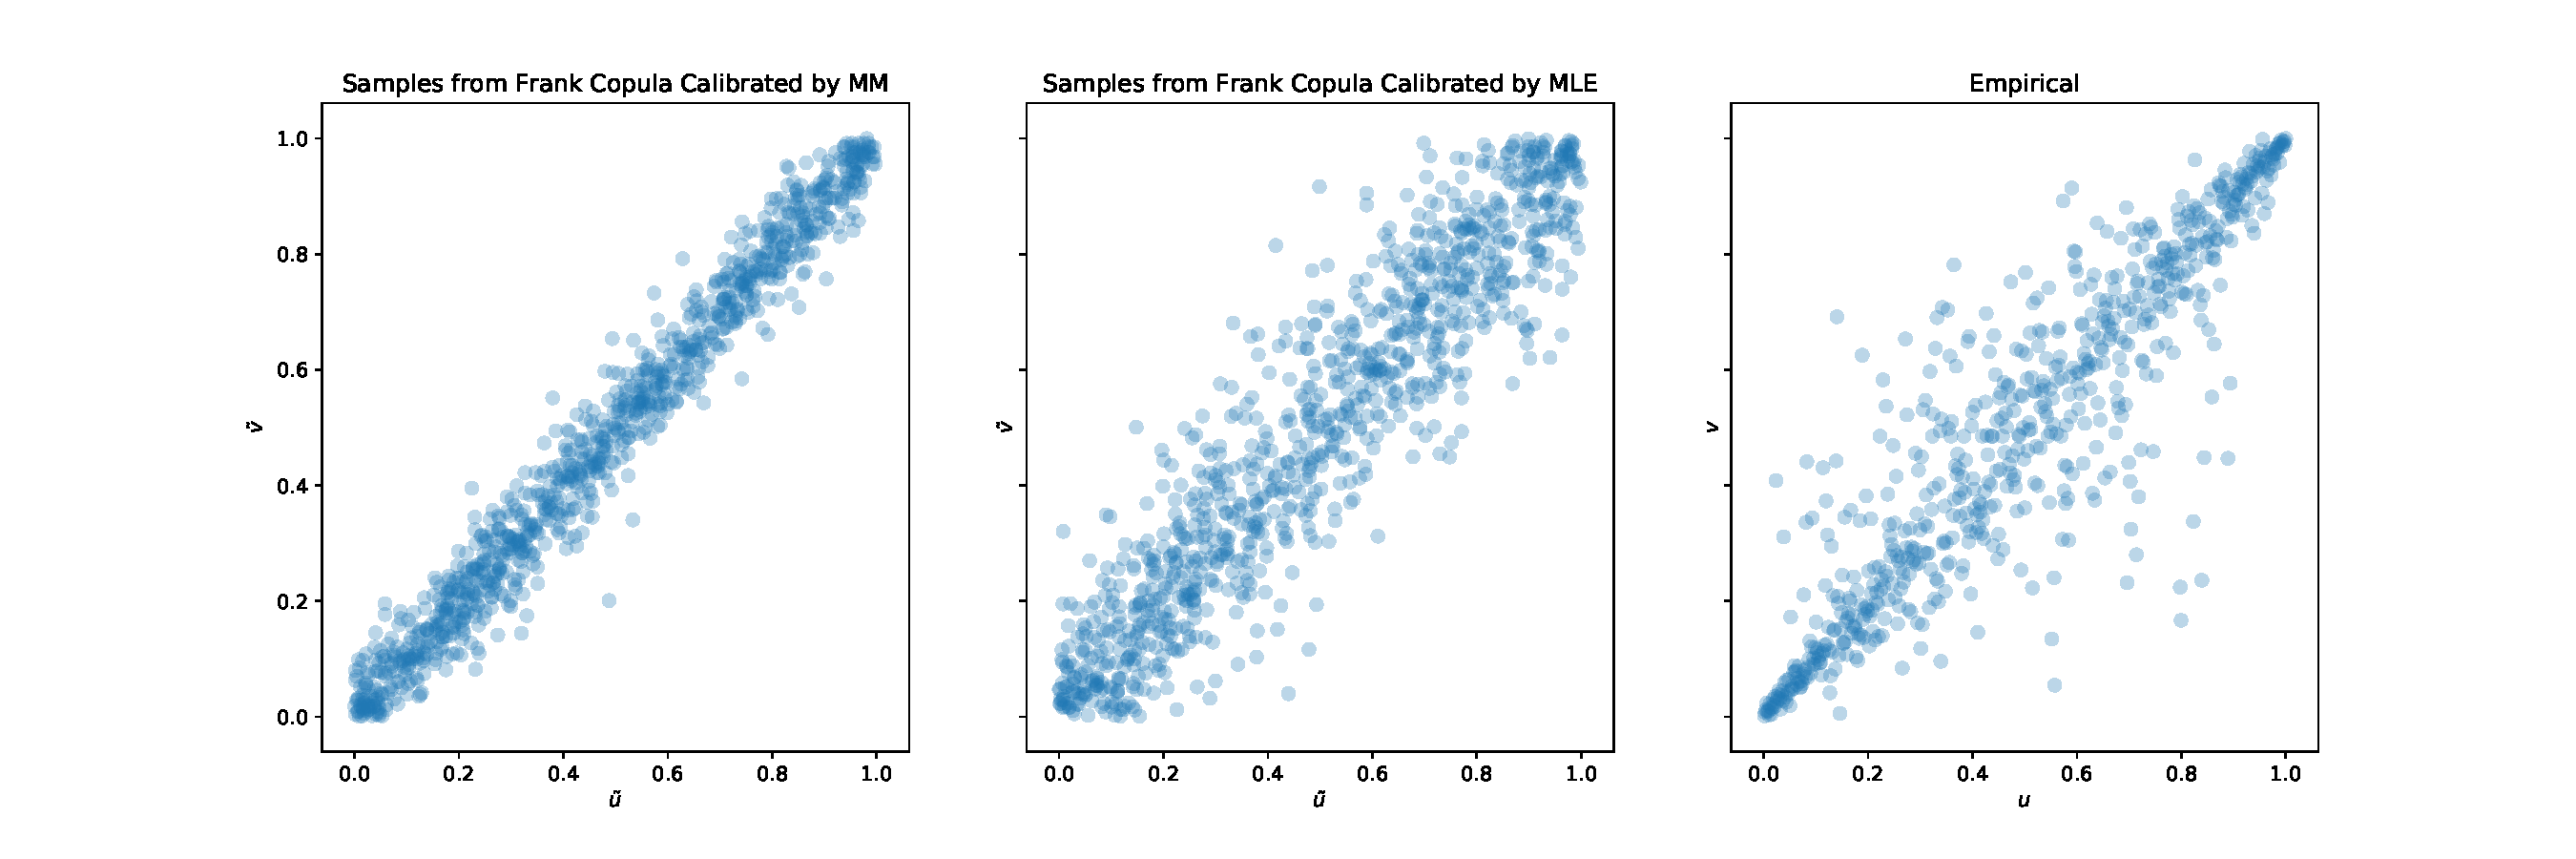
\includegraphics[width=\textwidth]{_pics/Frank.pdf}
   \caption{Comparison of Frank Copula Samples and Pseudo Observations of Bitcoin and CME Future Returns.
   \href{http://www.quantlet.com/}{
\includegraphics[width=20pt]{_pics/qletlogo_tr.png}}}
   \label{fig:Frank}
\end{figure}

Aside from the Frank-copula, the HEs of various combination of copula and risk reduction objective are very similar.
This is an expected result as the portfolio consists only two assets.
In addition to hedging effectiveness, we observe the out-of-sample returns of the hedged portfolio.
Figure~\ref{fig:OOSRH} tabulates the time series of out-of-sample returns of hedged portfolio under various copulas and risk reduction objectives.

One can see all the combinations of copula and risk reduction objective generate a large fluctuation of returns in
25/09/2019 and 26/09/2019.
This large fluctuation is due to dependence break.
\medskip

\begin{figure}[th]
   \centering
   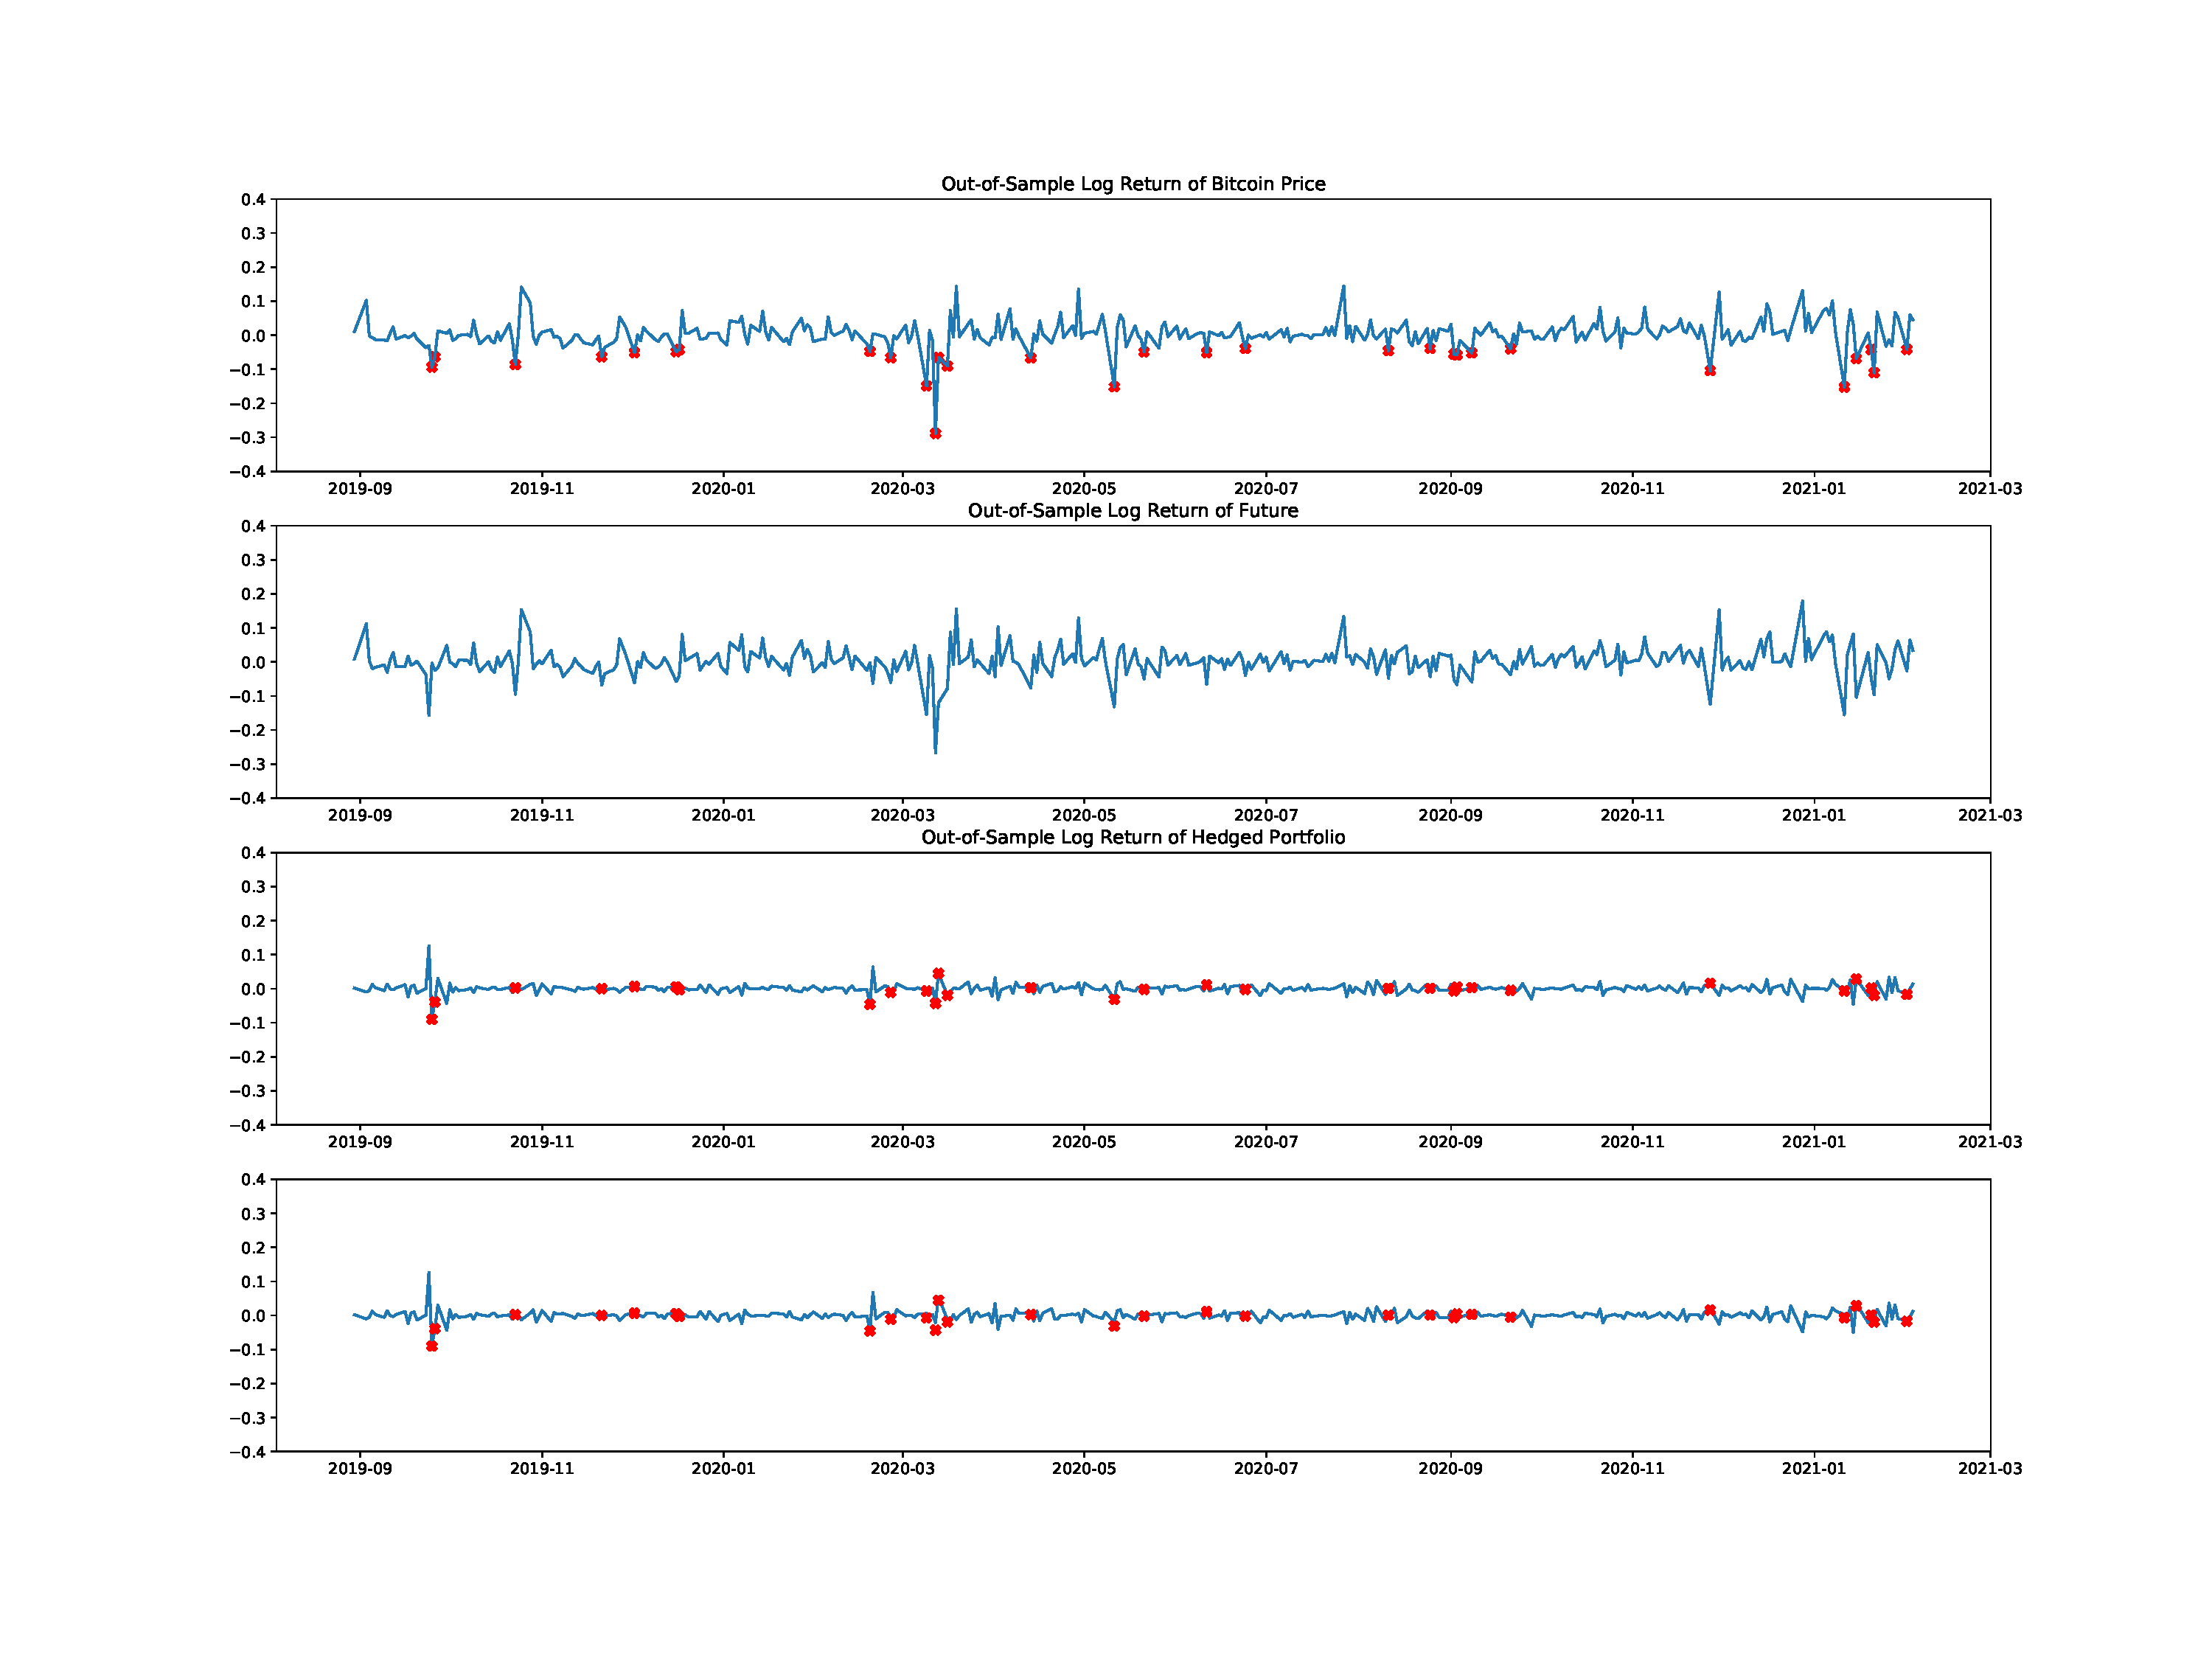
\includegraphics[width=\textwidth]{_pics/OOSreturns_compare.pdf}
   \caption{Upper panel: Out of Sample Log-return of Bitcoin; Middle panel:Out of Sample Log-return of Future;
   Lower panel: Out of Sample Log-return of Hedged Portfolio by Gumbel with the aim of variance reduction.
   The red dots indicate the lowest 10\% return of Bitcoin.
%   Lower Panel: Out of Sample Hedged Portfolio log-returns.
%   The $h^*$ is obtained from Gumbel copula aiming at reducing variance.
%   The red dots indicate the 30 most extreme negative returns in Bitcoin.
   \href{http://www.quantlet.com/}{
\includegraphics[width=20pt]{_pics/qletlogo_tr.png}}}
   \label{fig:Gumbel}
\end{figure}

\newpage
\begin{landscape}
\begin{figure}[th]
   \centering
   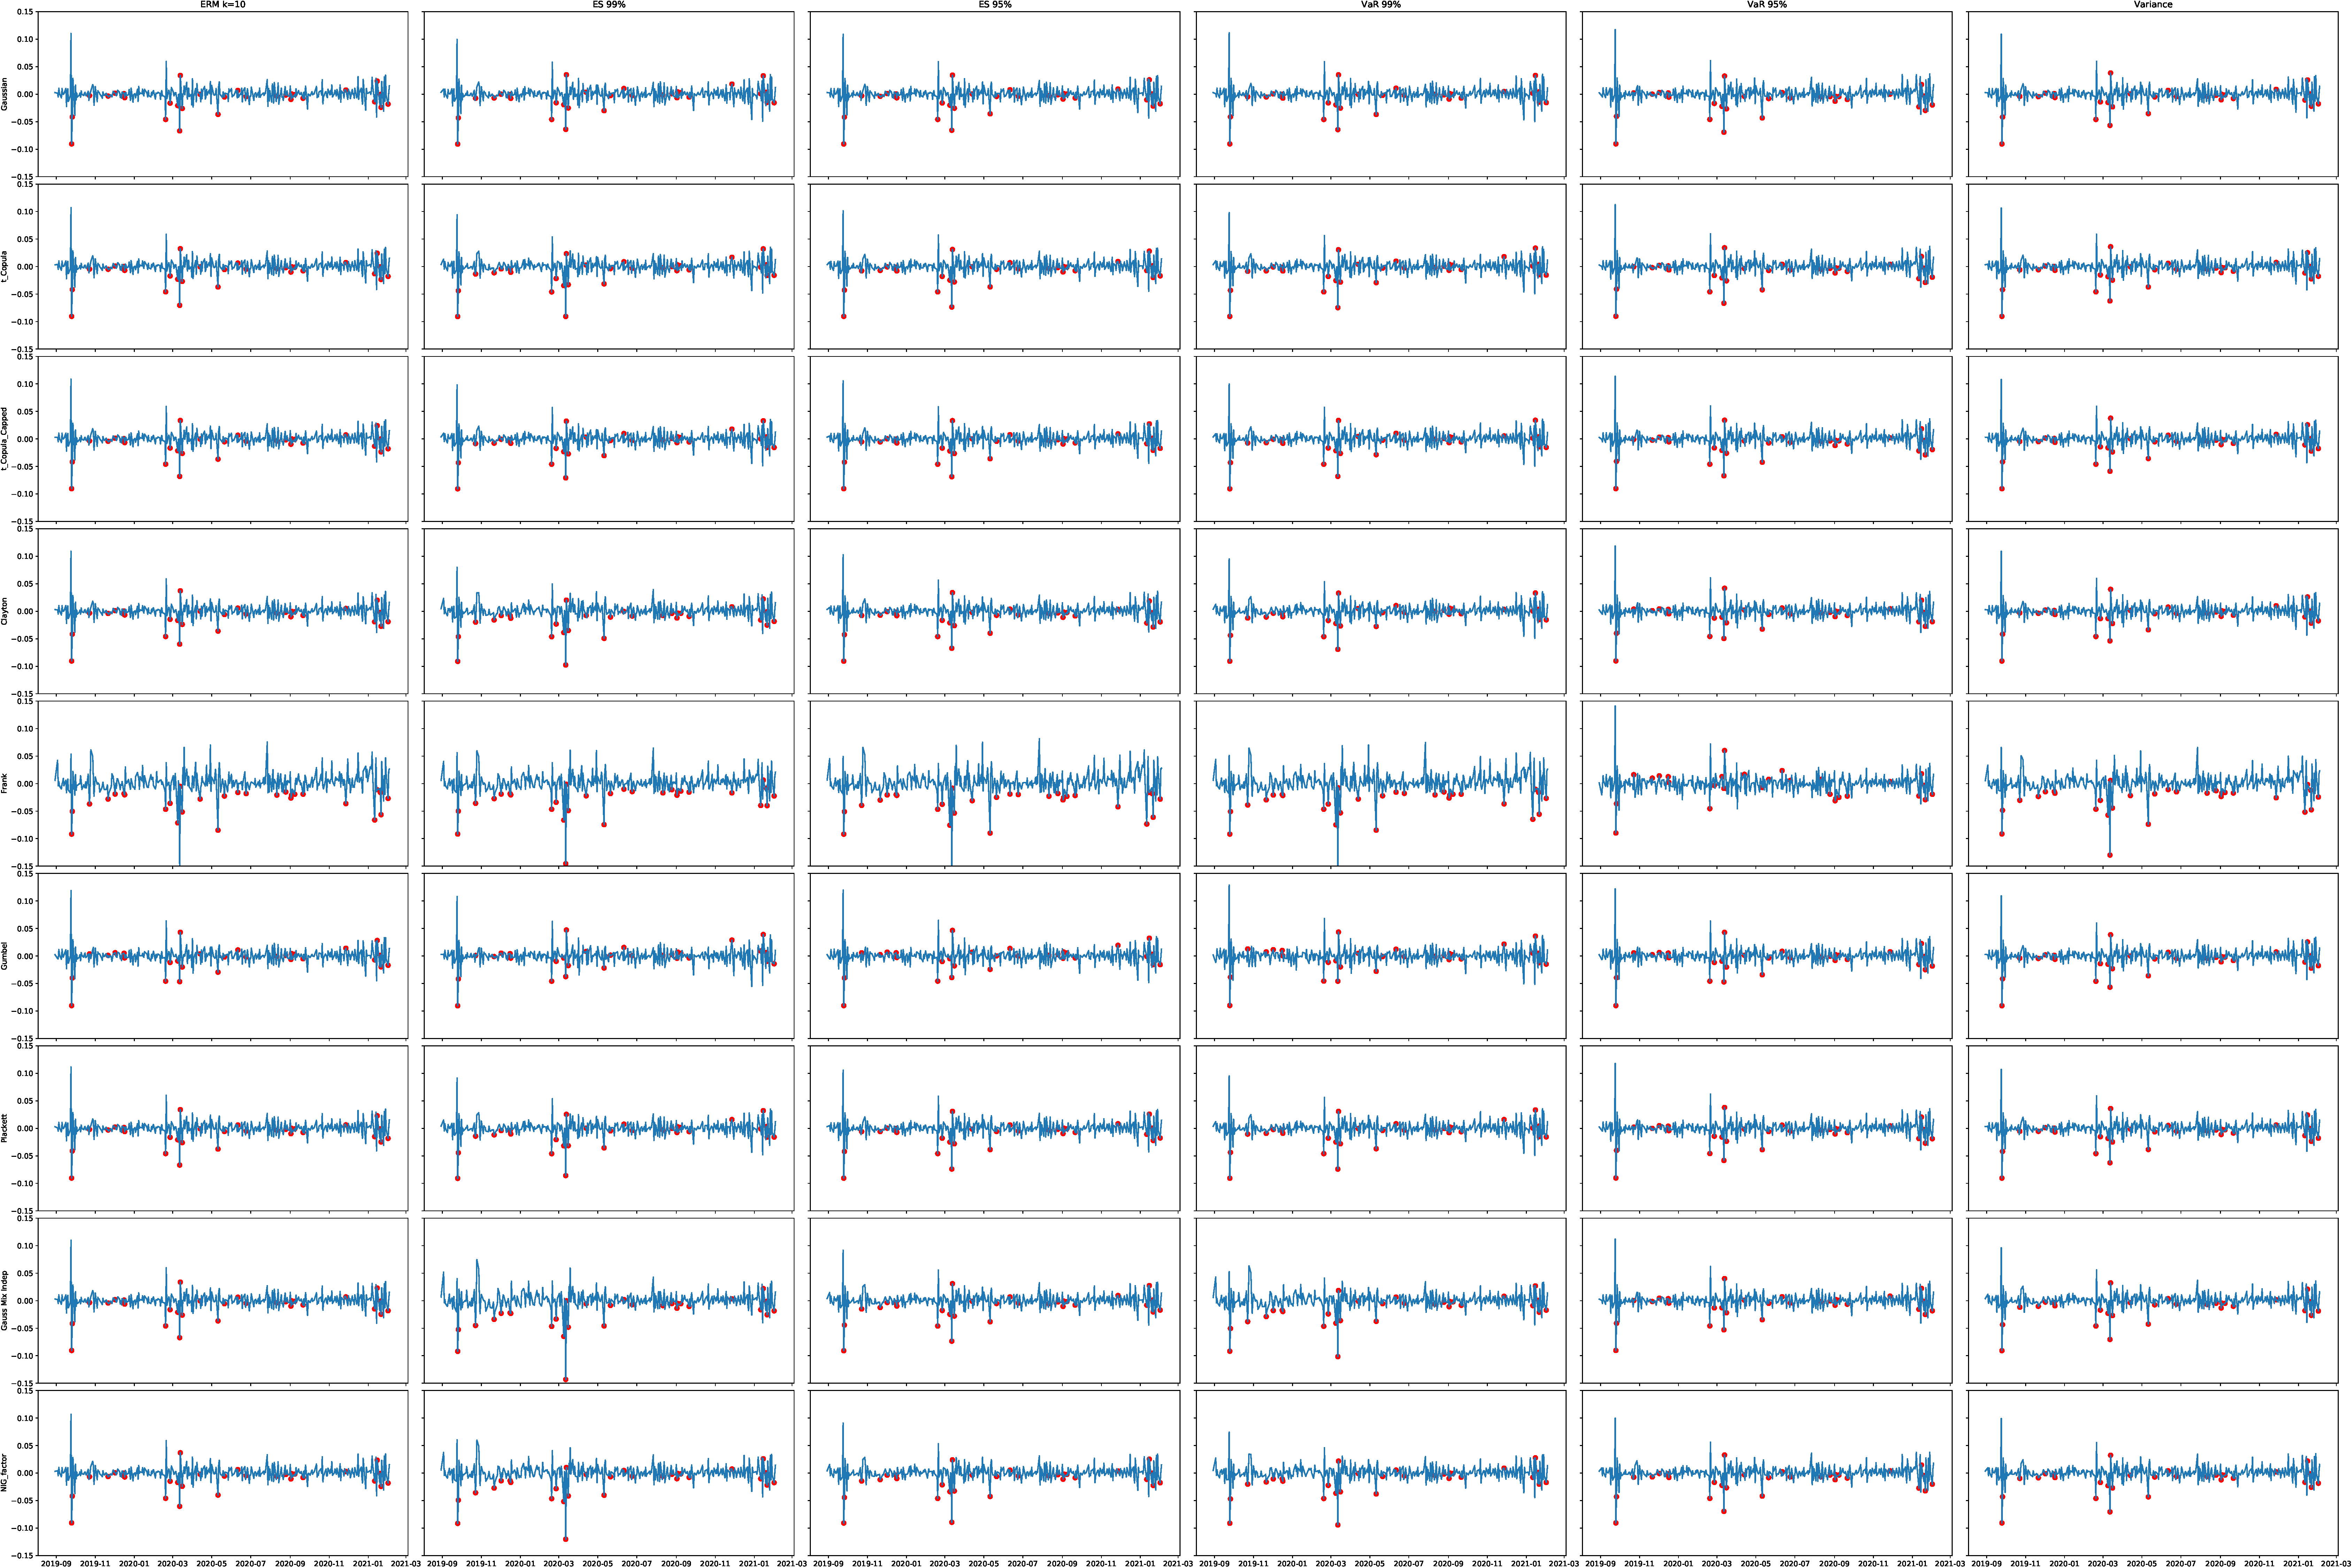
\includegraphics[width=\linewidth]{_pics/Rhs.pdf}
   \caption{Out-of-Sample Returns of Hedged Portfolio of Copulas and Risk Reduction Objectives.
   \href{http://www.quantlet.com/}{
\includegraphics[width=20pt]{_pics/qletlogo_tr.png}}}
   \label{fig:OOSRH}
\end{figure}
\end{landscape}
\newpage

\newpage
\begin{landscape}
\begin{figure}[th]
   \centering
   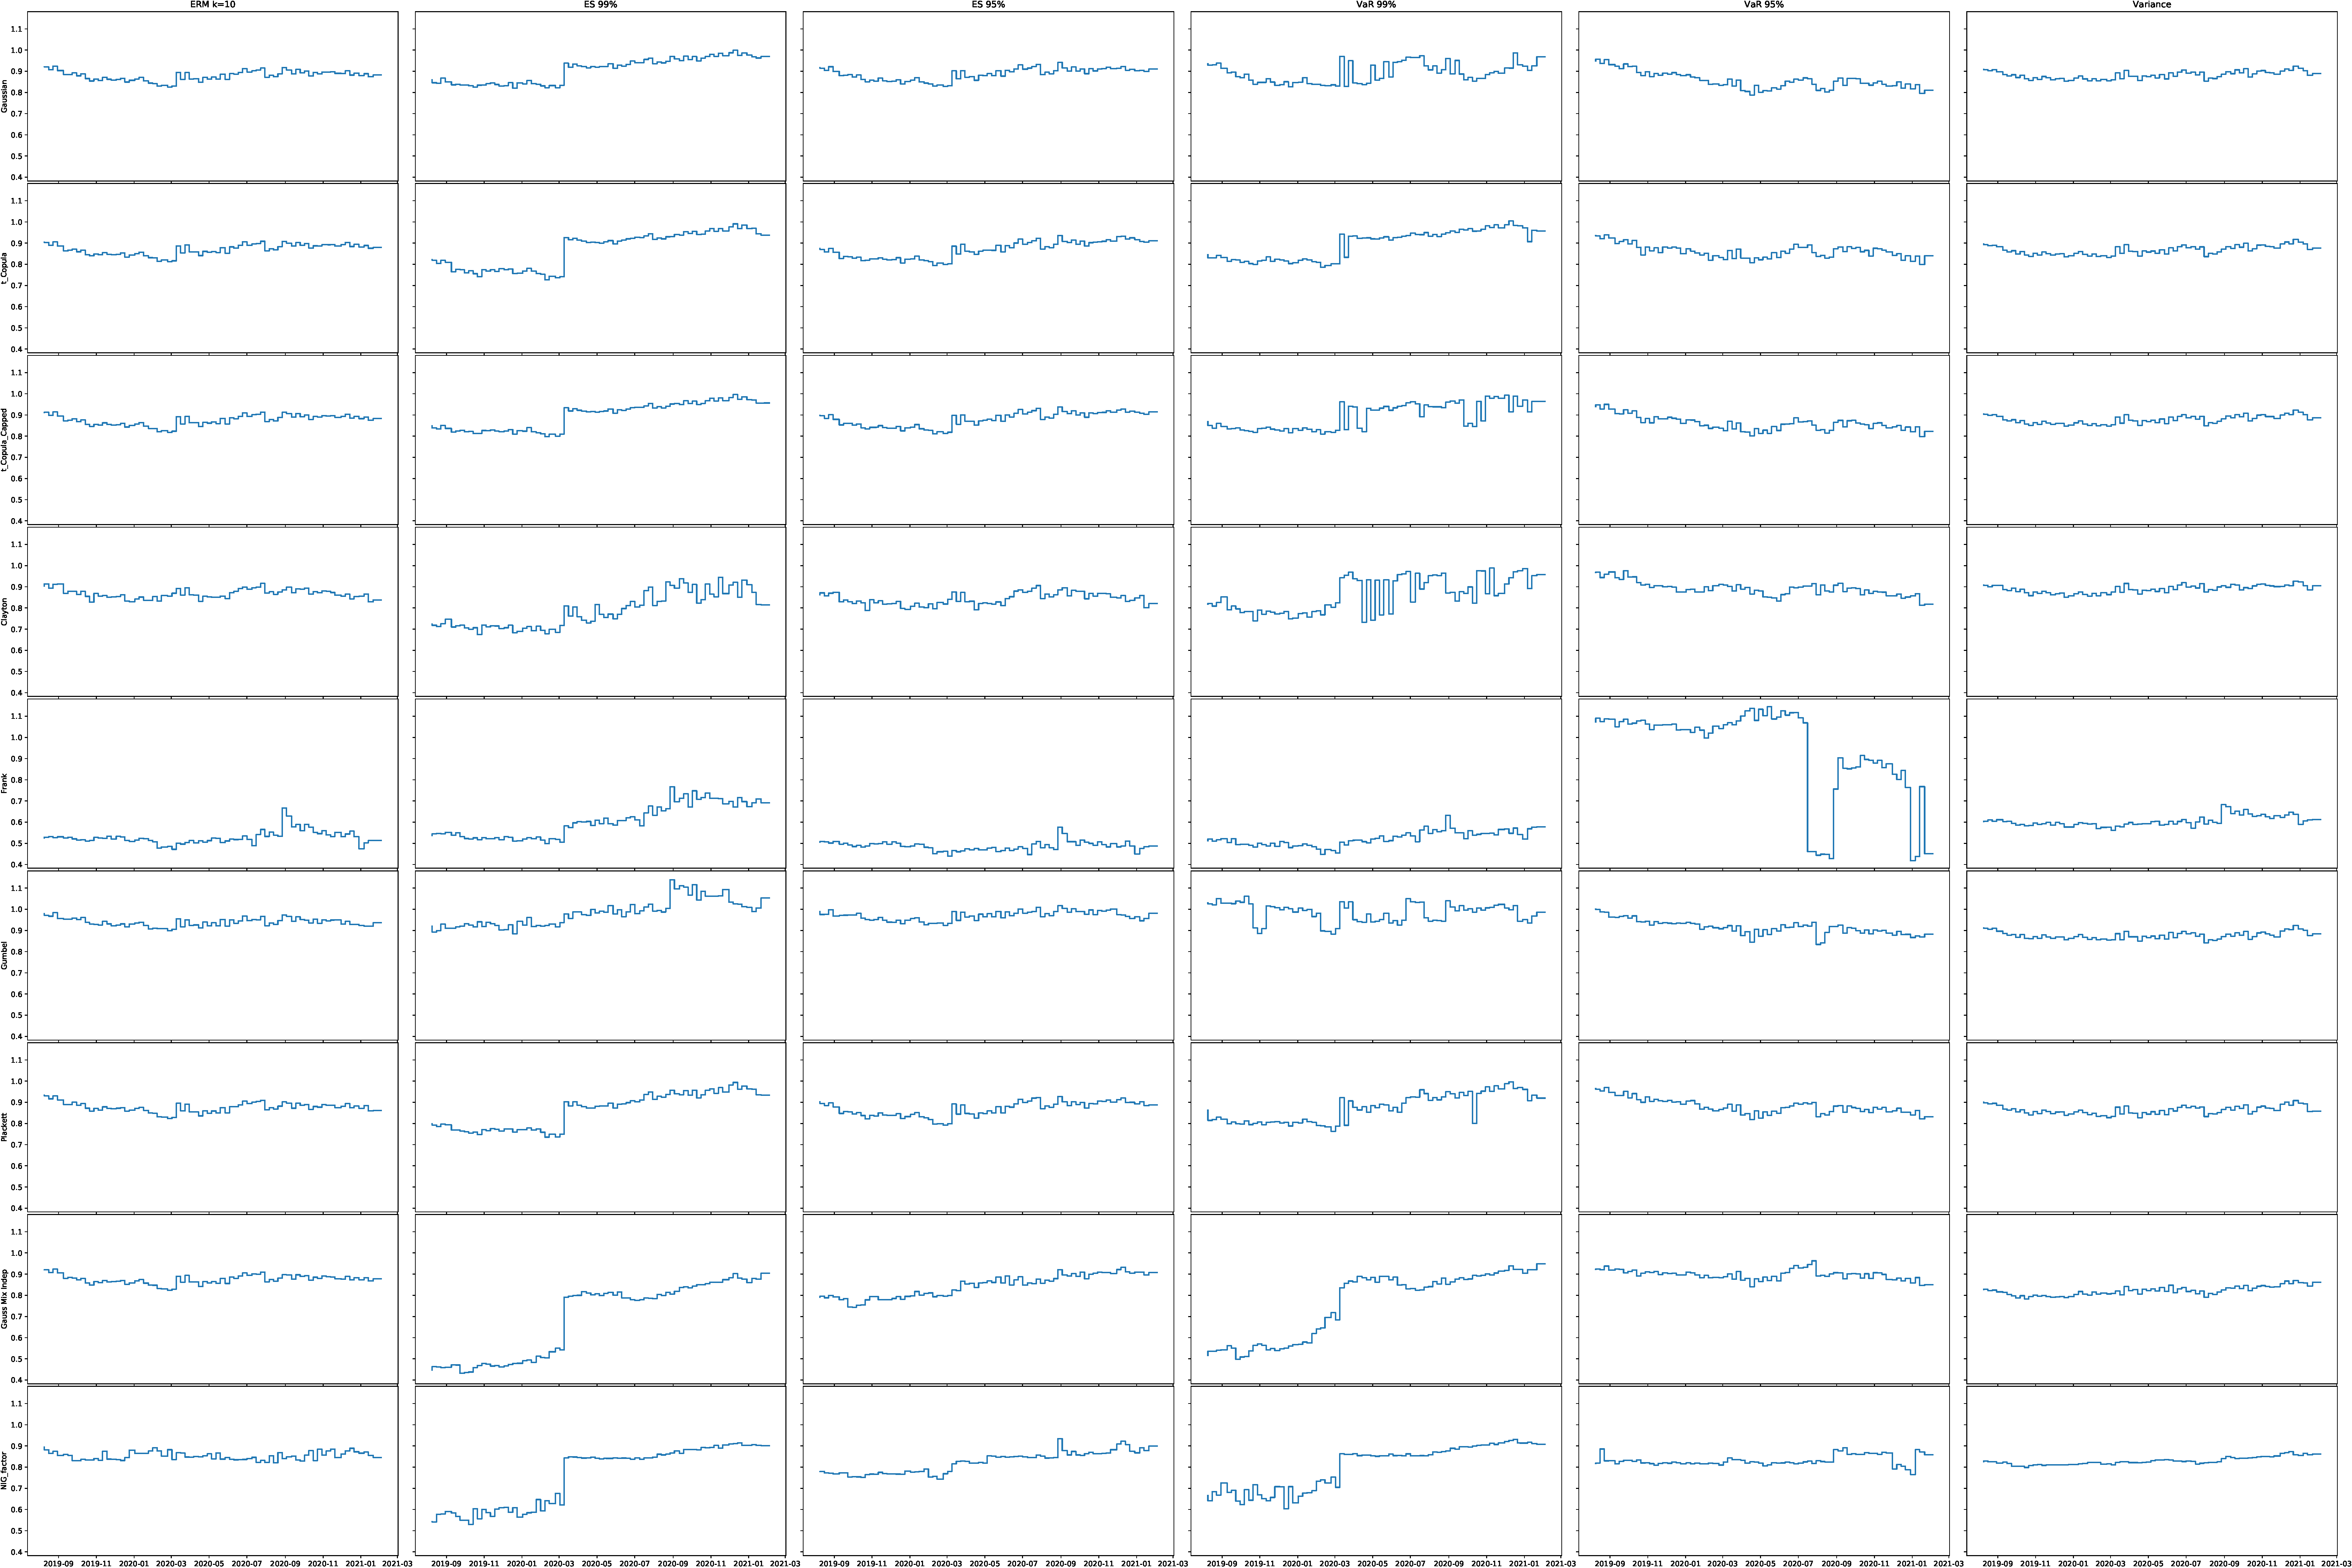
\includegraphics[width=\linewidth]{_pics/OHRs.pdf}
   \caption{Optimal Hedge Ratio Obtained from Combinations of Copula and Risk Reduction Objective.
   \href{http://www.quantlet.com/}{
\includegraphics[width=20pt]{_pics/qletlogo_tr.png}}}
   \label{fig:OHRs}
\end{figure}
\end{landscape}
\newpage


%\begin{figure}[t]
%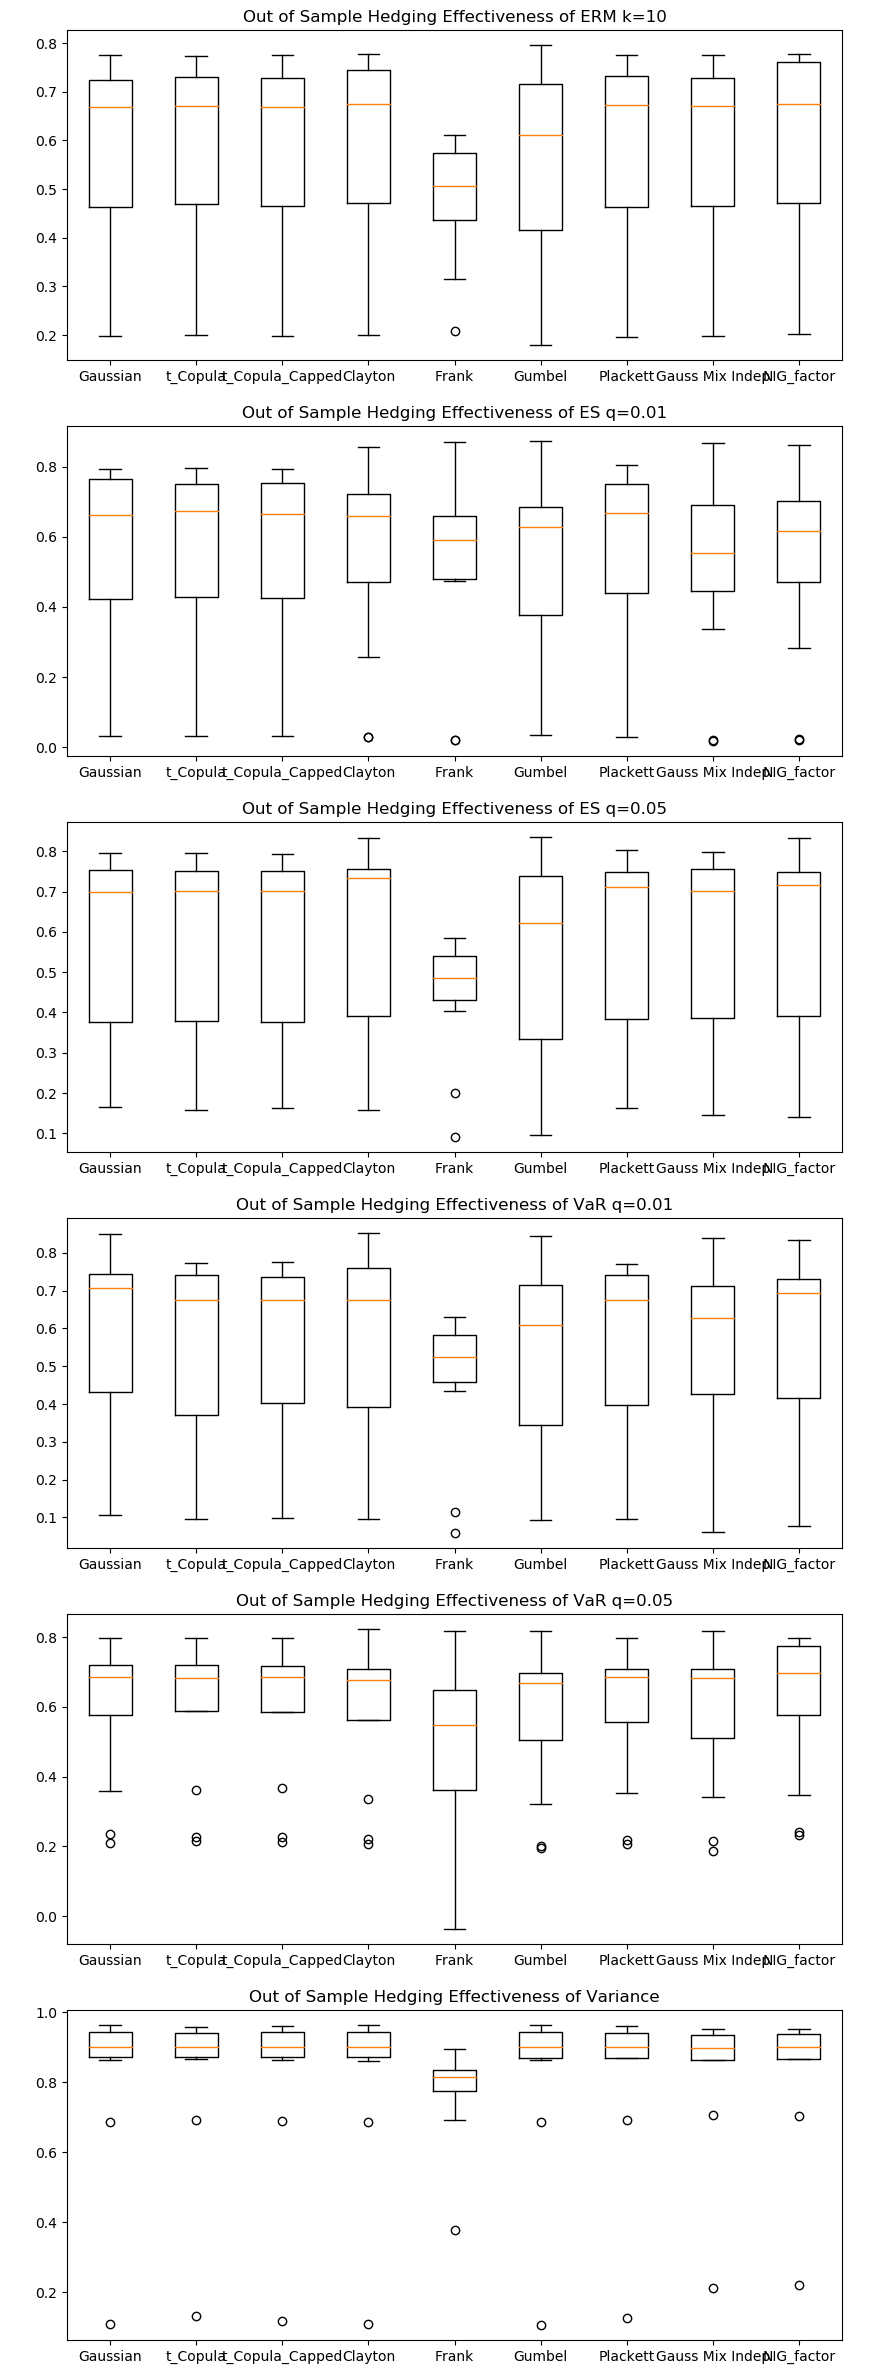
\includegraphics[width=\textwidth, height=\textheight]{_pics/Out of Sample Hedging Effectiveness.png}
%  \caption{}
%\label{out of Sample Hedging Effectieness}
%\end{figure}

\begin{figure}[!th]
   \centering
   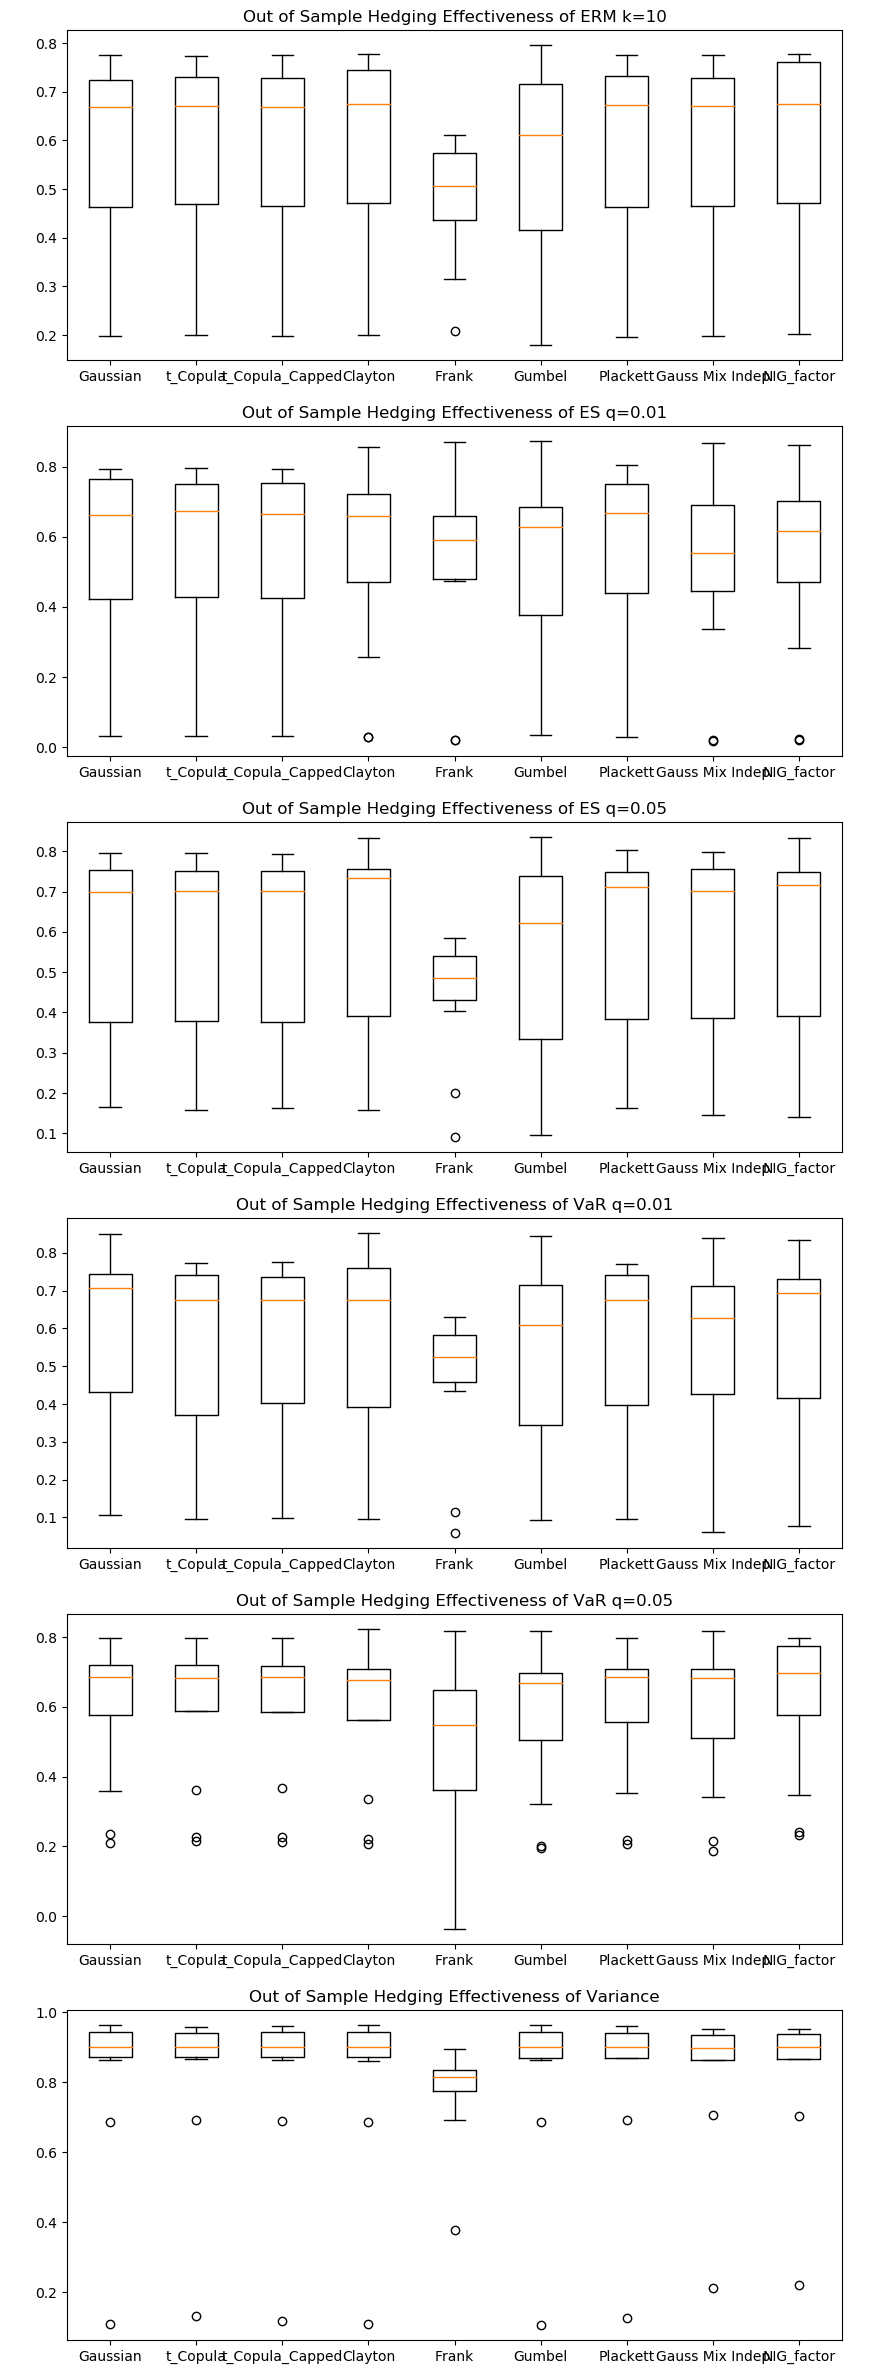
\includegraphics[height=25cm]{_pics/Out of Sample Hedging Effectiveness.png}
   \caption{Out of Sample Hedging Effectiveness Box-plot.
   The HEs are obtained from a set of out-of-sample data,
   each set consists 30 days log returns of Bitcoin and CME future.
   \href{http://www.quantlet.com/}{
\includegraphics[width=20pt]{_pics/qletlogo_tr.png}}}
   \label{fig:OOSHE}
\end{figure}

Figure~\ref{fig:Gumbel} shows the time series of out-of-sample $R^h$ using Gumbel copula with the
objective of reducing variance.
The red dots are the 30 most extreme negative returns in Bitcoin.
In the figure, we can see the downside risk of Bitcoin is well managed by the hedging procedure with Gumbel copula.
Most of the extreme losses of Bitcoin are greatly reduced by introducing the CME future in the hedged portfolio.
Two exceptions are found in 25/09/2019 and 26/09/2019, where the CME future failed to follow the large drop in Bitcoin. (TODO: drop reason)
One of the possible reason is that traders was performing rollover activities on 25-26/09/2019, which
27/09/2019 is the expiry day of the September future.
Another reason for Gumbel fail of capturing the loss is dependence break.
The Kendall's tau in the training data is 0.2 higher than that of the testing data.
Other copulas suffer from the break as well.



\subsection{Stability of $h^*$}
We measure the stability of $h^*$ by sum of absolute change
\begin{align}
    \sum_{t=1}^T|h_t - h_{t-1}|.
    \end{align}

Adjustment of portfolio weights induces price slippage (ref) and transaction cost.
From figure \ref{SAD} we know the NIG factor copula with variance as risk reduction objective generates the smallest
sum of absolute change in OHR.

\begin{figure}[!th]
   \centering
   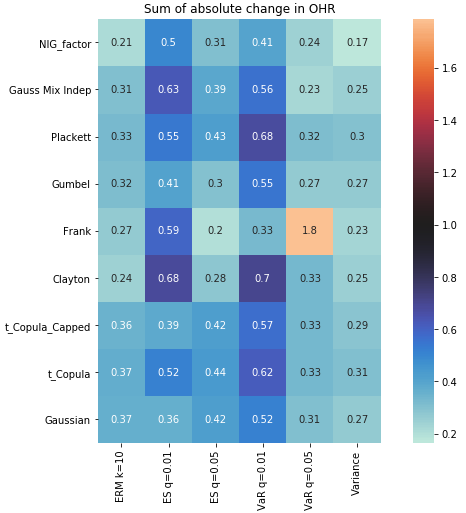
\includegraphics[width=\textwidth]{_pics/Sum of absolute change in OHR.png}
   \caption{Sum of Absolute Change in OHR.
   \href{http://www.quantlet.com/}{
\includegraphics[width=20pt]{_pics/qletlogo_tr.png}}}
   \label{fig:SAD}
\end{figure}

%%\usepackage{fontspec}
%\newcommand{\smallest}[1]{\textcolor{Maroon}{\textbf{#1}}}

\begin{table}
\begin{tabular}{lrrrrrr}
\toprule
{} &  ERM k=10 &    ES 99\% &    ES 95\% &   VaR 99\% &   VaR 95\% &  Variance \\
\midrule
Gaussian        &  0.019985 &  0.020802 &  0.020061 &  0.020230 &  0.019983 &  \color{blue}0.019757 \\
t\_Copula        &  0.020097 &  0.021698 &  0.020381 &  0.020966 &  0.020071 &  \color{blue}0.019890 \\
t\_Copula\_Capped &  0.020048 &  0.021018 &  0.020202 &  0.020554 &  0.020059 &  \color{blue}0.019792 \\
Clayton         &  0.019519 &  0.021341 &  0.019789 &  0.021045 &  \color{blue}0.019389 &  0.019675 \\
Frank           &  0.029234 &  0.026240 &  0.030770 &  0.029157 &  \color{blue}0.023085 &  0.025928 \\
Gumbel          &  0.020014 &  0.021411 &  0.020511 &  0.021643 &  \color{blue}0.019557 &  0.019757 \\
Plackett        &  0.020010 &  0.021531 &  0.020363 &  0.020870 &  \color{blue}0.019755 &  0.019909 \\
Gauss Mix Indep &  0.019949 &  0.025390 &  0.020454 &  0.023283 &  \color{blue}0.019667 &  0.020006 \\
NIG\_factor      &  \color{blue}0.019720 &  0.023425 &  0.020706 &  0.022039 &  0.019950 &  0.019999 \\
\bottomrule
\end{tabular}
\caption{Exponential Risk Measure $k=10$}
\end{table}

\begin{table}
\begin{tabular}{lrrrrrr}
\toprule
{} &  ERM k=10 &    ES 99\% &    ES 95\% &   VaR 99\% &   VaR 95\% &  Variance \\
\midrule
Gaussian        &  0.061084 &  0.062405 &  0.061201 &  0.062148 &  0.061712 &  \color{blue}0.059310 \\
t\_Copula        &  0.062148 &  0.068702 &  0.063339 &  0.063964 &  0.062067 & \color{blue}0.060735 \\
t\_Copula\_Capped &  0.061623 &  0.064114 &  0.062198 &  0.062466 &  0.062072 & \color{blue}0.059676 \\
Clayton         &  0.058495 &  0.069910 &  0.060812 &  0.064595 &  \color{blue}0.055962 &  0.058318 \\
Frank           &  0.104185 &  0.096795 &  0.108713 &  0.105070 &  \color{blue}0.068457 &  0.091321 \\
Gumbel          &  0.056513 &  0.059574 &  0.056035 &  0.058162 &  \color{blue}0.055492 &  0.059525 \\
Plackett        &  0.061167 &  0.068027 &  0.063426 &  0.064563 &  \color{blue}0.058491 &  0.061017 \\
Gauss Mix Indep &  0.061157 &  0.088023 &  0.063900 &  0.073316 &  \color{blue}0.057007 &  0.063081 \\
NIG\_factor      &  \color{blue}0.060878 &  0.078959 &  0.065270 &  0.070919 &  0.062097 &  0.062848 \\
\bottomrule
\end{tabular}
\caption{ES 99\%}
\end{table}

\begin{table}
\begin{tabular}{lrrrrrr}
\toprule
{} &  ERM k=10 &    ES 99\% &    ES 95\% &   VaR 99\% &   VaR 95\% &  Variance \\
\midrule
Gaussian        &  0.034488 &  0.035237 &  0.034548 &  0.035123 &  0.034838 &  \color{blue}0.034248 \\
t\_Copula        &  0.034777 &  0.037100 &  0.035234 &  0.035634 &  0.035055 &  \color{blue}0.034494 \\
t\_Copula\_Capped &  0.034647 &  0.035679 &  0.034862 &  0.035282 &  0.034937 &  \color{blue}0.034322 \\
Clayton         &  0.033714 &  0.037282 &  0.034230 &  0.036089 &  \color{blue}0.033445 &  0.034046 \\
Frank           &  0.053661 &  0.047849 &  0.056299 &  0.053409 &  \color{blue}0.037638 &  0.046953 \\
Gumbel          &  0.034028 &  0.035965 &  0.034528 &  0.036353 &  \color{blue}0.033568 &  0.034293 \\
Plackett        &  0.034592 &  0.036831 &  0.035316 &  0.035752 &  \color{blue}0.034186 &  0.034558 \\
Gauss Mix Indep &  0.034439 &  0.045160 &  0.035120 &  0.040027 &  \color{blue}0.033756 &  0.034478 \\
NIG\_factor      &  \color{blue}0.033882 &  0.041001 &  0.035677 &  0.037975 &  0.034656 &  0.034453 \\
\bottomrule
\end{tabular}
\caption{ES 95\%}
\end{table}

\begin{table}
\begin{tabular}{lrrrrrr}
\toprule
{} &  ERM k=10 &    ES 99\% &    ES 95\% &   VaR 99\% &   VaR 95\% &  Variance \\
\midrule
Gaussian        &  \color{blue}0.041327 &  0.044416 &  0.041943 &  0.043399 &  0.042275 &  0.041981 \\
t\_Copula        &  \color{blue}0.041450 &  0.044830 &  0.042806 &  0.043789 &  0.041693 &  0.041969 \\
t\_Copula\_Capped &  \color{blue}0.041498 &  0.044169 &  0.042411 &  0.044051 &  0.042018 &  0.042056 \\
Clayton         &  \color{blue}0.040022 &  0.044523 &  0.042878 &  0.044215 &  0.040913 &  0.041943 \\
Frank           &  0.076644 &  0.055387 &  0.081273 &  0.073433 &  \color{blue}0.046177 &  0.061056 \\
Gumbel          &  0.042079 &  0.042139 &  0.042187 &  0.045340 &  \color{blue}0.040523 &  0.041937 \\
Plackett        &  \color{blue}0.041013 &  0.044971 &  0.042370 &  0.042995 &  0.041574 &  0.041731 \\
Gauss Mix Indep &  0.040998 &  0.048017 &  0.043249 &  0.044518 &  \color{blue}0.040749 &  0.043386 \\
NIG\_factor      &  \color{blue}0.040457 &  0.047201 &  0.043925 &  0.044230 &  0.043240 &  0.043138 \\
\bottomrule
\end{tabular}
\caption{VaR 99\%}
\end{table}

\begin{table}
\begin{tabular}{lrrrrrr}
\toprule
{} &  ERM k=10 &    ES 99\% &    ES 95\% &   VaR 99\% &   VaR 95\% &  Variance \\
\midrule
Gaussian        &  0.020385 &  0.020315 &  0.020143 &  0.020412 &  0.020121 &  \color{blue}0.019579 \\
t\_Copula        &  0.020547 &  0.020428 &  0.020661 &  0.020611 &  0.020370 &  \color{blue}0.019820 \\
t\_Copula\_Capped &  0.020525 &  0.020544 &  0.020503 &  0.020486 &  0.020224 &  \color{blue}0.019656 \\
Clayton         &  0.019702 &  0.021042 &  0.020143 &  0.020640 &  0.019990 &  \color{blue}0.019700 \\
Frank           &  0.026372 &  0.023529 &  0.027105 &  0.026212 &  \color{blue}0.023389 &  0.023594 \\
Gumbel          &  0.019781 &  0.021311 &  0.020716 &  0.020421 &  \color{blue}0.019077 &  0.019541 \\
Plackett        &  0.020459 &  0.020257 &  0.020589 &  0.020100 &  0.020237 &  \color{blue}0.020047 \\
Gauss Mix Indep &  0.020482 &  0.024753 &  0.020304 &  0.024158 &  \color{blue}0.019944 &  0.020723 \\
NIG\_factor      &  \color{blue}0.019923 &  0.023784 &  0.021009 &  0.022172 &  0.019980 &  0.020670 \\
\bottomrule
\end{tabular}
\caption{VaR 95\%}
\end{table}

\begin{table}
\begin{tabular}{lrrrrrr}
\toprule
{} &  ERM k=10 &    ES 99\% &    ES 95\% &   VaR 99\% &   VaR 95\% &  Variance \\
\midrule
Gaussian        &  0.014387 &  0.014380 &  0.014360 &  0.014530 &  0.014670 &  \color{blue}0.014294 \\
t\_Copula        &  0.014378 &  0.014626 &  0.014343 &  0.014385 &  0.014627 &  \color{blue}0.014306 \\
t\_Copula\_Capped &  0.014375 &  0.014418 &  0.014332 &  0.014430 &  0.014643 &  \color{blue}0.014290 \\
Clayton         &  0.014306 &  0.014870 &  0.014332 &  0.014532 &  0.014493 &  \color{blue}0.014267 \\
Frank           &  0.021495 &  0.018982 &  0.022736 &  0.021476 &  \color{blue}0.018142 &  0.018897 \\
Gumbel          &  0.014618 &  0.014971 &  0.014878 &  0.015438 &  0.014622 &  \color{blue}0.014321 \\
Plackett        &  0.014444 &  0.014560 &  0.014424 &  0.014423 &  0.014596 &  \color{blue}0.014353 \\
Gauss Mix Indep &  0.014404 &  0.017404 &  \color{blue}0.014341 &  0.015671 &  0.014453 &  0.014408 \\
NIG\_factor      &  \color{blue}0.014362 &  0.015841 &  0.014484 &  0.015043 &  0.014474 &  0.014415 \\
\bottomrule
\end{tabular}
\caption{Standard Deviation}
\end{table}